%%
%% $Id$
%%
%% Copyright (c) 2007-2008 Christian Fehler
%% Copyright (c) 2007-2008 Benjamin Mies
%%


\chapter{Automaten}\label{Machines}

Im Mittelpunkt der Planung und der Umsetzung des \gtitools standen die Automaten.
Im Rahmen dieser Diplomarbeit wurden vier Automatentypen umgesetzt. Der
deterministische endliche Automat (DEA), der nicht determinitische endliche
Automat (NDEA), der $\epsilon$ nicht deterministische endliche Automat
($\epsilon$-NDEA) und schließlich der Kellerautomat. Die verschiedenen Aspekte
von Automaten werden in diesem Kapitel besprochen, dazu gehört die graphische
Umsetzung, sowie die verschiedenen Möglichkeiten, diesen zu verwenden, wenn er
angelegt wurde.\vspace{10pt}


\section{Graphenansicht}\label{Graph}

In diesem Abschnitt wird die Graphendarstellung besprochen. Zu Beginn der
Diplomarbeit wurde diskutiert, welche Möglichkeiten zur Darstellung eines
Automaten zur Verfügung stehen. Im Raum standen das eigenständige
Implementieren der graphischen Komponenten, sowie die Verwendung einer
Bibliothek, die diese Funktionalität zur Verfügung stellt. Aufgrund des
vermutlich enormen Zeitaufwandes wurde entschieden, eine Bibliothek zu benutzen.
In Abschnit \ref{PerspectiveGraphics} wird darauf eingegangen, in wie weit eine
Änderung in Zukunft sinnvoll bzw. realisierbar wäre.\vspace{10pt} 

%### removes texlipse warning
Da JGraph (siehe \cite{jgraph}) die benötigte Funktionalität zur Verfügung
stellt, um die Automaten darstellen zu können, wurde entschieden, diese
Bibliothek zu benutzen. Im Folgenden wird darauf eingegangen, wie Automaten mit
JGraph dargestellt werden und wie JGraph angepasst werden musste, um den
speziellen Ansprüchen unserer Umsetzung zu genügen.\vspace{10pt}
%### removes texlipse warning


\subsection{Automatendarstellung mit JGraph}\label{GraphJGraph}

%### removes texlipse warning
Bei der Darstellung der Automaten haben wir uns sehr daran orientiert, wie sie
hier \cite{Sieber} verwendet wird. Wir wollten eine möglichst hohe Überdeckung
erreichen, um sicherzustellen, dass ein Benutzer einen existierenden Automaten
verstehen kann, ohne sich noch viel einlesen zu müssen. In den
Vorlesungsunterlagen wird ein Zustand als Kreis dargestellt. Ein akzeptierender
Zustand wird über einen doppelten Rahmen gekennzeichnet. Einen Startzustand
erkennt man an einem Pfeil, wlecher mit Start beschriftet ist.\vspace{10pt}
%### removes texlipse warning

\begin{figure}[h!]
\begin{center}
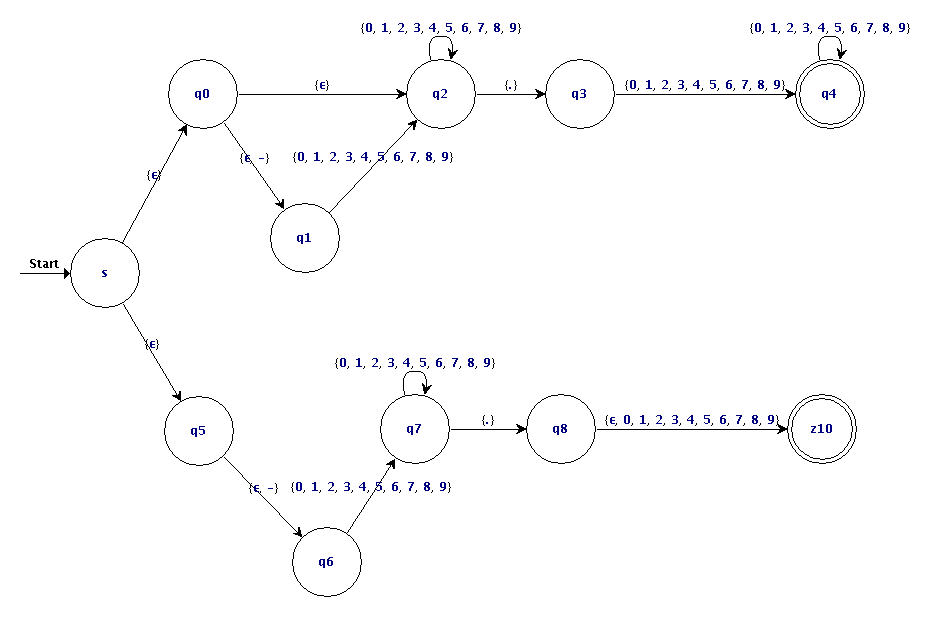
\includegraphics[width=12cm]{../images/enfa_example.png}
\caption{Beispiel für eine Automatendarstellung mit JGraph}
\end{center}
\end{figure}
\vspace{10pt}

Als erstes mussten wir mit Hilfe von JGraph Komponenten eine geeignete
Darstellung von Zuständen und Übergängen erreichen. Diese Komponenten mussten dynamisch
angelegt, gelöscht und bearbeitet werden können. Nachdem wir also eine passende
Darstellung für unsere Automaten gefunden hatten, mussten wir noch die
Verknüpfung von den graphischen Elementen und den Kernelementen herstellen. Um
eine eindeutige Zuweisung von diesen Elementen zu erreichen, haben wir uns dazu
entschieden, die Kernelemente als Attribut in den graphischen Komponenten zu
speichern.\vspace{10pt}

Nachdem die Verknüpfung der Komponenten erledigt war, konnte man die Darstellung
der Zustände und Übergänge anhand der entsprechenden Daten anpassen. Das bedeutet
für Zustände, dass man den Namen des Zustandsobjekts anzeigt, und auch auswertet,
ob es sich um einen Startzustand oder um einen Endzustand handelt. Bei den
Übergängen konnte die Übergangsmenge als Beschriftung benutzt werden, wie es bei
der Vorlage im Skript der Fall ist.\vspace{10pt}


\subsection{Anpassung von JGraph}\label{GraphJGraphAdaptation}

Die Bibliothek JGraph bietet eine weit über unsere Anforderungen hinaus
gehende Unterstützung von graphischen Komponenten. An einigen Stellen mussten
allerdings Anpassungen vorgenommen werden, um den von uns vorgegebenen
Funktionumfang erreichen zu können. Diese Anpassungen werden in diesem
Abschnitt geschildert.\vspace{10pt}

Als erste Anpassung wurde umgesetzt, dass die Farbe der Zustände geändert
werden kann. Dies wird zwar von der Bibliothek unterstützt, allerdings wurde
von uns eine Verknüpfung mit den Kernelementen gewünscht. Auf diese Weise ist
es nun möglich, einem solchen Kernelement zu sagen, dass es aktiv oder
fehlerhaft ist. Die graphische Komponente aktualisiert sich dann beim nächsten
Zeichnen automatisch. Durch diese Art der Implementierung ist es jetzt sehr
einfach, in den verschiedenen Algorithmen die Darstellung der graphischen
Komponenten zu beeinflussen.\vspace{10pt}

Eine weitere Anpassung, die von uns implementiert wurde, ist die schon von den
Parsern, siehe Kapitel \ref{Parser}, bekannte Verwendung von sogenannten
PrettyStrings. Bei einfachen Übergängen oder Zuständen mit kurzem Namen
beinhaltet diese Anpassung nicht allzu viele Verbesserungen. Das sieht bei der
Verwendung von mehreren Symbolen in einem Übergang oder den
Potenzmengen-Zuständen anders aus. Dort ist der Benutzer in der Lage, durch die
zu\-sätz\-lich\-en Farbinformationen und Zeichenattribute, die ihm zur Verfügung
gestellten Informationen schneller aufzunehmen, als wenn ihm eine unformatierte
Zeichenkette angezeigt werden würde.\vspace{10pt}

In Kapitel \ref{ConverTo} wird die Umwandlung von Automaten in andere Automaten-
Formen, z.B. die Umwandlung von einem $\epsilon$-NDEA in einen DEA besprochen.
Bei der Implementierung dieser Umwandlung wurden wir vor das Problem gestellt,
dass in der Literatur, sowie im Vorlesungsskript, Potenzautomaten-Zustände nicht
rund dargestellt werden, sondern als Rechteck mit abgerundeten Ecken. Dieses
Problem wurde durch die Anpassung der graphischen Zustände, sowie durch die
Berechnung der Endpunkte der Übergänge gelöst.\vspace{10pt}

Die Darstellungsweise von parallelen Übergängen in entgegengesetzte Richtung
musste angepasst werden, da die normale Implementierung ein Ergebnis lieferte,
das dem als Vorlage benutzten Beispiel im Vorlesungsskript nicht ähnlich
war.\vspace{10pt}

Die letzte wichtige Anpassung wurde notwendig, da ein Start-Zustand mit einem
Pfeil auf den Zustand dargestellt werden musste. Dieser graphische Pfeil musste
somit zu dem Zustand gehören, was die Breite des Zustandes erhöhte und damit die
normale Berechnung von JGraph, zum Beispiel die Berechnung der Position eines
Überganges beeinflusste und dafür sorgte, dass der Graph nicht mehr so aussah,
wie er intuitiv aussehen sollte. Um dieses Problem zu lösen, musste bei vielen
Berechnungen, ein Offset berücksichtigt werden, so dass ein Start-Zustand nicht
mehr anders behandelt wurde, wie ein normaler Zustand.\vspace{10pt}


\section{Tabellen}\label{Tables}

In diesem Abschnitt werden die zwei Tabellen beschrieben, die bei den Automaten
verwendet werden, um dem Benutzer zusätzliche Informationen zur Verfügung zu
stellen. Die Übergangstabelle bietet zusätzlich noch die Möglichkeit, den
Automaten zu verändern. Es können Übergänge angelegt, modifiziert oder gelöscht
werden.\vspace{10pt}


\subsection{Übergangstabelle}\label{TablesTransition}

Während der Entwicklung und ersten Tests des \gtitools kam der Wunsch auf, einen
Automaten nicht nur graphisch zu bearbeiten, sondern auch in der
Übergangstabelle. Dadurch soll es dem Benutzer ermöglicht werden, Übergänge
schneller anzulegen, als es bei der normaler Methode in der Graphenansicht der
Fall wäre. Um diese neue Methode zu implementieren, wurden verschiedene
Umsetzungen diskutiert. Zur Diskussion standen unter anderem, dass in jeder Zelle
der Tabelle ausgewählt werden kann, zu welchen Zuständen ein Übergang existiert.
Diese Auswahl hätte allerdings bei der graphiscnen Umsetzung Probleme bereitet,
zumindest bei hinreichend vielen Zuständen. Aus diesem Grund wurde dieser Ansatz
verworfen.\vspace{10pt}

\begin{figure}[h!]
\begin{center}
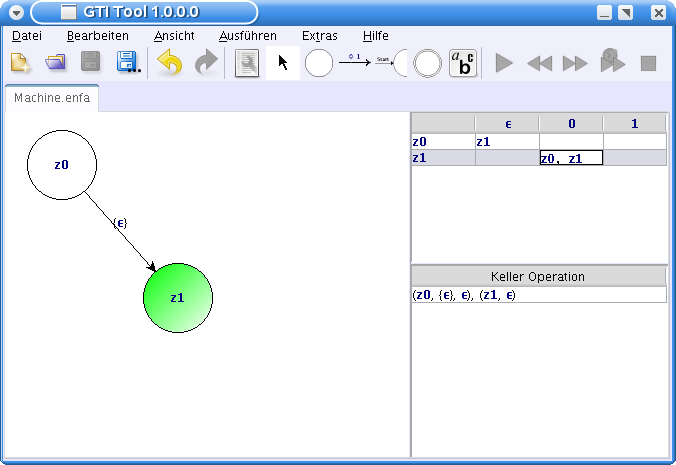
\includegraphics[width=12cm]{../images/machine_table.png}
\caption{Übergangstabelle}
\label{FigureMachineTable}
\end{center}
\end{figure}
\vspace{10pt}

Als nächste mögliche Umsetzung wurde diskutiert, ob es technisch möglich sei,
in jeder Zelle einen Parser zu verwenden. Dieser Parser müsste so implementiert
werden, dass er einen oder mehrere, durch Kommata getrennte Zustände als Eingabe
akzeptiert. Im Kapitel \ref{Parser} werden einige kontextsensitive Bedingungen
angesprochen, die auch bei dem hier vorliegenden Parser verwendet werden
mussten, da es dem Benutzer nicht möglich sein sollte, einen oder mehrere
Zustände anzugeben, die nicht im Graphen vorkommen. Abbildung
\ref{FigureMachineTable} zeigt das von uns umgesetzte Ergebnis.\vspace{10pt}


\subsection{Keller Operationen Tabelle}\label{TablesPDA}

Anhand der Tabelle für Kelleroperationen kann der Benutzer genau
nachvollziehen, was genau mit dem Keller des Automaten passiert, wenn wir
in einen anderen Zustand übergehen.\vspace{10pt}

\begin{figure}[h!]
\begin{center}
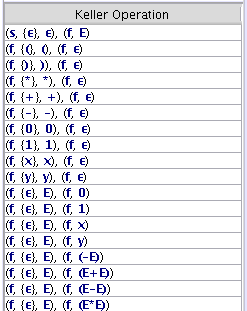
\includegraphics[width=12cm]{../images/stack_operation_table.png}
\caption{Keller Operationen Tabelle}
\label{FigureStackOperationTable}
\end{center}
\end{figure}
\vspace{10pt}

Die Tabelle enthält einen Eintrag pro Übergang in unserem Automaten. Jeder
Eintrag enthält den Zustand von dem der Übergang ausgeht, den Zustand zu dem
wir übergehen und die entsprechende Übergangsmenge. Zusätzlich wird noch
das Wort angegeben, welches bei diesem Übergang vom Keller gelesen wird, und
das Wort, welches auf den Keller geschrieben wird. Wenn wir nichts vom
Keller lesen, oder auf den Keller schreiben, wird als Wort "`$\epsilon$"'
verwendet.\vspace{10pt} 

In Abbildung \ref{FigureStackOperationTable} sieht man, wie eine
solche Tabelle aussehen kann.\vspace{10pt}


\section{Wort-Navigation}\label{WordNavigation}

In diesem Abschnitt wird die Wort-Navigation beschrieben. Neben der
deterministischen Navigation wird das Anzeigen des Pfades zu den aktuell
aktiven Zuständen angesprochen, das dem Benutzer erleichtern soll, zu
verstehen, warum ein eingegebenes Wort erkannt wird.


\subsection{Deterministische Navigation}\label{WordNavigationDeterministic}

Wir wollten dem Nutzer auch die Möglichkeit geben, sich anzusehen, wie der
konstruierte Automat ein beliebiges Eingabewort abarbeitet. Dabei muss es sich
um ein gültiges Wort über dem Alphabet handeln. Für diesen Zweck wurde die
Wort-Navigation entwickelt.\vspace{10pt}

Wenn der Nutzer den Wort-Navigationsmodus startet, findet er am unteren
Bildschirmrand zwei Textfelder. Hierbei handelt es sich um ein Eingabefeld für
das Eingabewort, und um eine Anzeige des aktuellen Kellers. In der
deterministischen Wort-Navigation spielt die Kelleranzeige keine Rolle. Diese
wird allerdings bei der Verwendung von einem Kellerautomaten benötigt und wird
in Abschnitt \ref{InteractionPDA} besprochen.\vspace{10pt}

Um dem Benutzer eine Hilfestellung bei der Eingabe eines Wortes zu geben, wird
rechts neben dem Eingabefeld das aktuelle Alphabet angezeigt. Man kann nur
Symbole verwenden, welche auch im Eingabealphabet enthalten
sind.\vspace{10pt}

\begin{figure}[h]
\begin{center}
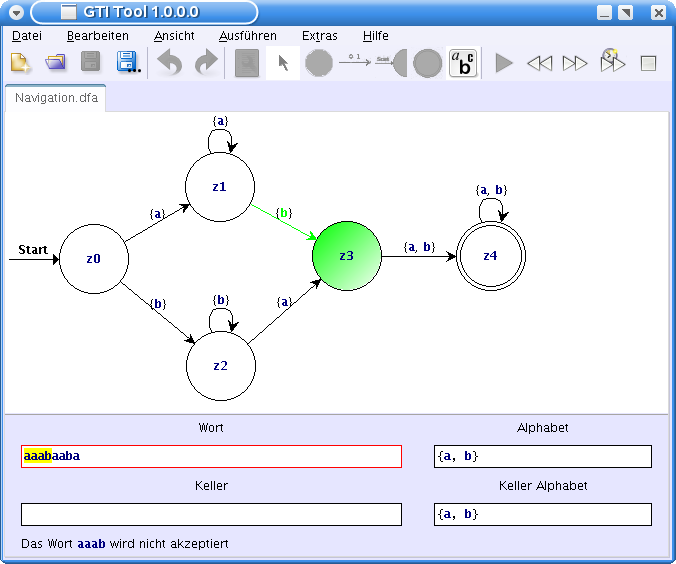
\includegraphics[width=12cm]{../images/dfa_navigation.png}
\caption{Automat - Wort-Navigation}
\end{center}
\end{figure}
\vspace{10pt}

Nachdem ein Wort eingegeben wurde, kann der Nutzer dann die Verarbeitung des
Worts starten. Es besteht die Möglichkeit, sich Zeichen für Zeichen weiter durch
das Wort zu arbeiten, und den genauen Weg im Automaten nachzuvollziehen.\vspace{10pt}

In jedem Schritt werden die Zustände farblich hervorgehoben, in denen sich der
Automat aktuell befindet. Zusätzlich wird auch der Übergang und das
entsprechende Symbol des Übergangs hervorgehoben, über welchen man in diesen
Zustand gekommen ist. In dem Feld, in welchem man das Wort eingegeben hat, wird
jetzt angezeigt, bis zu welcher Stelle der Automat das Wort schon verarbeitet
hat.\vspace{10pt}

Wenn man das ganze Wort gelesen hat, bekommt der Benutzer eine Information,
ob der Automat das Wort akzeptiert hat, oder, ob das Wort nicht in der Sprache
liegt, welche von dem Automaten erkannt wird.\vspace{10pt}


\subsection{Zustands Pfad}\label{HistoryPath}

Bei Verwendung eines nicht deterministischen Automaten stellte sich bei der
Wort-Navigation die Frage, auf welchem Pfad die aktuell aktiven Zustände erreicht
wurden. Verschiedene Umsetzungen wurden von uns qin Betracht gezogen, um dem
Benutzer die Ausgabe darzustellen. Es wurde schließlich entschieden, die Zustände
auf dem Pfad zu den aktuell aktiven Zuständen darzustellen. Auf diesem Pfad
werden die verwendeten Übergänge, sowie die verwendeten Symbole an den Übergängen
hervorgehoben. Da unter Umständen mehrere Pfade vorhanden sein können, werden
diese anhand der Anzahl der verwendeten Zustände sortiert, dabei werden die
kürzesten Pfade zuerst angezeigt.\vspace{10pt}

\begin{figure}[h!]
\begin{center}
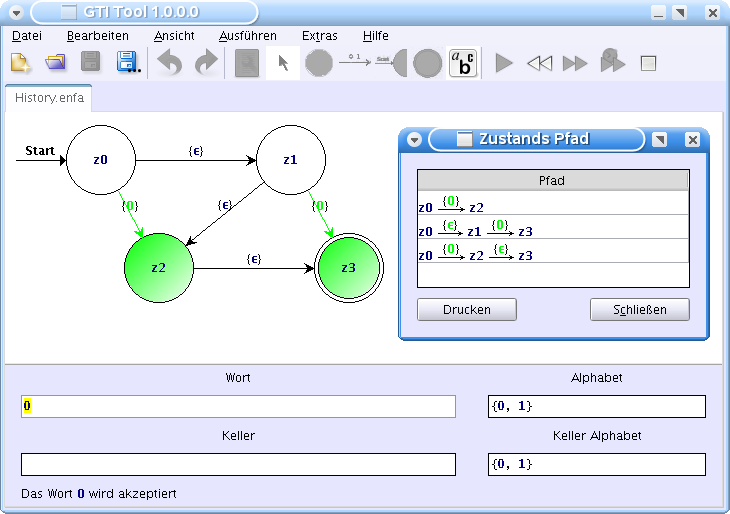
\includegraphics[width=12cm]{../images/history_path.png}
\caption{Zustands Pfad}
\end{center}
\end{figure}
\vspace{10pt}

Der implementierte Algorithmus geht rückwärts vor, startet also bei den aktuell
aktiven Zuständen und geht alle Pfade zurück, bis alle, beim Starten der Ansicht
vom Eingabewort gelesenen Symbole abgearbeitet sind. Startet der berechnete Pfad
dann in dem Startzustand, wurde ein gültiger Pfad erkannt. Bei der
Implementierung des Algorithmus musste eine Zykluserkennung umgesetzt werden, da
es sonst möglich wäre, in eine Endlosschleife zu geraten, welche durch
$\epsilon$-Übergänge verursacht wurde.\vspace{10pt}


\section{Erreichbare Zustände}\label{ReachableStates}

Nach dem in \ref{ConverToMachine} nachzulesenen Umwandeln eines nicht
deterministischen in einen deterministischen Automaten unter Verwendung der
Potenzautomatenkonstruktion stellte sich die Frage, wie die unerreichbaren
Zustände erkannt und entfernt werden können. Dieses Problem betrifft aber nicht
nur umgewandelte Automaten, sondern ganz allgemein, jeden erstellten
Automaten.\vspace{10pt}

Bei der Umsetzung sollte im Vordergrund stehen, dass dem Benutzer mit sehr
kleinen Schritten verdeutlicht wird, wie der zugrundeliegende Algorithmus
arbeitet, so dass diese Arbeitsweise sehr einfach nachzuvollziehen
ist.\vspace{10pt}

%### removes texlipse warning
Zur Umsetzung wurde der in \cite[S. 536]{Algorithmen} angegebene Algorithmus
als Vorlage benutzt. Dieser Algorithmus implementiert die Breitensuche auf
einem Graphen G mit Startknoten s. Zur Interpretation des Algorithmus ist noch
zu sagen, dass das Attribut Farbe eines Knoten dazu verwendet wird, zu
speichern, in welcher Phase des Algorithmus er sich befindet. Ist ein Knoten
weiß, bedeutet das, dass er noch nicht erkannt wurde. Am Anfang sind alle
Knoten, außer dem Startknoten, weiß. Grau bedeutet, dass der Knoten erkannt
wurde, aber noch nicht vollständig abgearbeitet wurde. Wurde ein Knoten
abgearbeitet, ändert sich seine Farbe in schwarz. Bei der Umsetzung im \gtitool
wurde eine ähnliche Umsetzung gewählt, die nun dargestellt wird.\vspace{10pt}
%### removes texlipse warning

\noindent
\verb| 1 BFS(G,s)|\\
\verb| 2 for alle Knoten u |$\in$\verb| V[G] - {s}|\\
\verb| 3     do farbe[u] |$\gets$\verb| WEISS|\\
\verb| 4        d[u] |$\gets \infty$\\
\verb| 5        |$\pi$\verb|[u] |$\gets$\verb| NIL|\\
\verb| 6 farbe[s] |$\gets$\verb| GRAU|\\
\verb| 7 d[s] |$\gets$\verb| 0|\\
\verb| 8 |$\pi$\verb|[s] |$\gets$\verb| NIL|\\
\verb| 9 Q |$\gets \emptyset$\\
\verb|10 ENQUEUE(Q,s)|\\
\verb|11 while Q |$\neq \emptyset$\\
\verb|12       do u |$\gets$\verb| DEQUEUE(Q)|\\
\verb|13          for alle v |$\in$\verb| Adj[u]|\\
\verb|14              do if farbe[v] = WEISS|\\
\verb|15                    then farbe[v] |$\gets$\verb| GRAU|\\
\verb|16                         d[v] |$\gets$\verb| d[u] + 1|\\
\verb|17                         |$\pi$\verb|[v] |$\gets$\verb| u|\\
\verb|18                         ENQUEUE(Q,v)|\\
\verb|19          farbe[u] |$\gets$\verb| SCHWARZ|\\
\vspace{10pt}

Der dann im Programm umgesetzte Algorithmus besteht aus drei Phasen.

In der ersten Phase wird ein noch nicht abgearbeiteter Zustand ausgewählt, also
ein Zustand, der von einem anderen Zustand aus erreichbar ist, aber für den noch
nicht berechnet wurde, welche Zustände von ihm aus erreichbar sind. Zu Beginn des
Algorithmus wird mit dem Startzustand angefangen. In der zweiten Phase werden die
von diesem Zustand aus direkt erreichbaren Zustände berechnet und dem Benutzer
hervorgehoben dargestellt. In der dritten Phase werden alle bis jetzt
erreichbaren Zustände hervorgehoben. Gleichzeitig wird rechts in der Outline
angezeigt, welcher Zustand jetzt fertiggestellt ist und welche noch berechnet
werden müssen. Durch diese sehr feine Unterteilung soll ein besseres Verständnis
des Algorithmus erreicht werden.\vspace{10pt}

\begin{figure}[h!]
\begin{center}
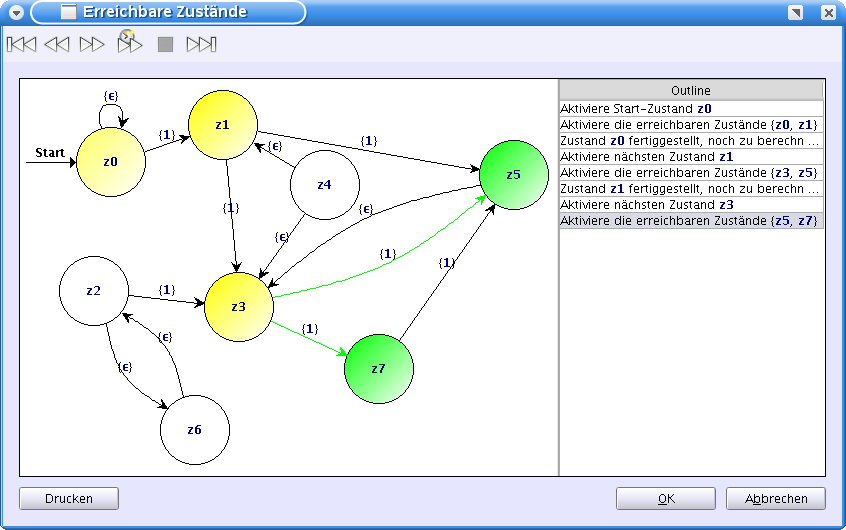
\includegraphics[width=12cm]{../images/reachable_states.png}
\caption{Erreichbare Zustände}
\end{center}
\end{figure}
\vspace{10pt}
